\documentclass[]{beamer}
\usepackage[T1]{fontenc}
\usepackage[utf8]{inputenc}
\usepackage{lmodern}
\usepackage[italian]{babel}
\usepackage{mathrsfs}
\usepackage{cancel}
\usepackage{multicol}

\title{La Fisica e il linguaggio matematico}
\author{\texorpdfstring{Mattia Cozzi\newline\href{mailto:cozzimattia@gmail.com}{\texttt{cozzimattia@gmail.com}}}{Mattia Cozzi}}
\date{a.s.~2023/2024}

%\documentclass[handout]{beamer}     %usare questa classe per generare l'handout
%\usepackage{pgfpages}   %per mostrare più quadri nella stessa pagina
%\pgfpagesuselayout{4 on 1}[a4paper,border shrink=5mm,landscape]
\usetheme{Singapore}
%\useoutertheme[left]{sidebar} %elementi intorno alle diapositive
\setbeamercovered{dynamic} %modifica l'aspetto del testo grigetto delle diapositive future. Argomenti: invisible/transparent/dynamic
\usecolortheme{orchid}
%COLORE PRINCIPALE
% \definecolor{marroncino}{RGB}{156, 26, 0} % UBC Blue (primary)
% \setbeamercolor{structure}{fg=marroncino} % itemize, enumerate, etc

\usepackage{tikz}
\usepackage{circuitikz}

\usepackage{pgf,pgfplots,graphicx}
\usetikzlibrary{angles,quotes,arrows,shapes,decorations.markings}
\pgfplotsset{compat=1.15}
\usepgfplotslibrary{units,fillbetween} % to add units easily to axis

\newcommand{\fem}{f_{em}}

\def\angolo[#1](#2)(#3:#4:#5)% Syntax: [draw options] (center) (initial angle:final angle:radius)
    { \draw[#1] ($(#2)+({#5*cos(#3)},{#5*sin(#3)})$) arc (#3:#4:#5); }


\begin{document}

\begin{frame}
  \titlepage
\end{frame}





\begin{frame}
\frametitle{Contenuti}
\tableofcontents
\end{frame}

\section{Intro}


\begin{frame}
\frametitle{Cosa è la Fisica?}
La Fisica (dal greco ``$ \varphi \upsilon \sigma \iota \varsigma $'', \emph{physis}, natura) è la scienza che \alert<1>{studia e descrive i fenomeni naturali},{\pause} riproducendoli, quando possibile, con \alert<2>{esperimenti},{\pause} osservandone risultati e \alert<3>{misurando le grandezze} che li determinano,{\pause} allo scopo di individuare le relazioni tra queste grandezze e \alert<4>{le leggi che governano i fenomeni}.{\pause}

~

Alle sue basi stanno il \alert<5>{metodo sperimentale} e osservativo{\pause} e la formalizzazione di tali leggi tramite il \alert<6>{linguaggio matematico}.
\end{frame}


\begin{frame}
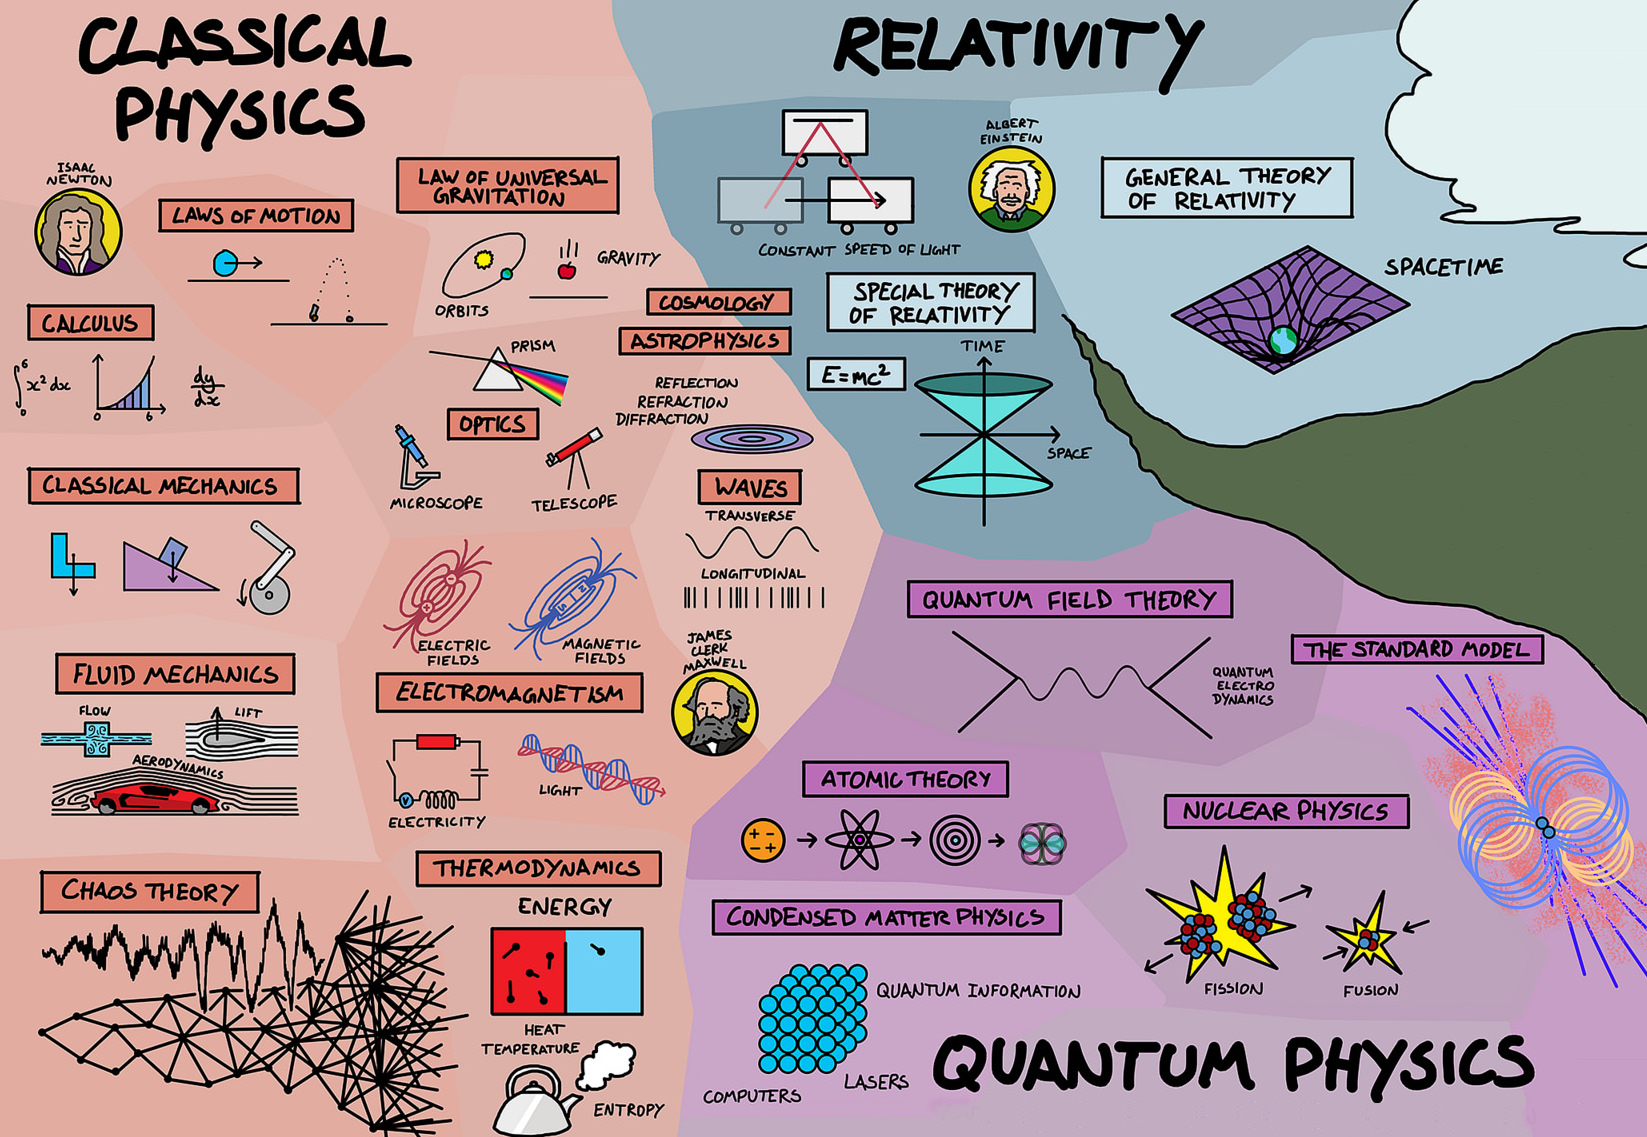
\includegraphics[width=\columnwidth]{img/mappafisica.jpg}
\end{frame}




\begin{frame}
\frametitle{Il linguaggio matematico e il suo utilizzo}
Il linguaggio matematico è il miglior linguaggio per la Fisica:
\begin{itemize}
  \item \alert<1>{non presenta ambiguità};\pause
  \item \alert<2>{è identico per tutti} i suoi utilizzatori;\pause
  \item esprime precisamente \alert<3>{i rapporti che sussistono tra le quantità};\pause
  \item permette di effettuare \alert<4>{calcoli e deduzioni}.\pause
\end{itemize}

~

Conoscere e saper utilizzare tale linguaggio è necessario per poter comprendere e fare Fisica.
\end{frame}

\section{Misura}

\begin{frame}
\frametitle{Misura}
In Fisica frasi come:
\begin{multicols}{3}
  \begin{center}
    `Sono alto $ 1,75 $.'
    
    `È dimagrito di $ 2 $.'
    
    `Il video dura $ 24 $.'
    \end{center}
\end{multicols}
non hanno alcun senso! {\pause}

~

Per esprimere una misura sono infatti necessari \alert<2>{un numero} e una \alert<2>{unità di misura}.\pause

~

Dal 1961 è in uso il \alert<3>{Sistema Internazionale delle unità di misura (SI)}, che comprende udm utilizzate universalmente.\pause

~

Diremo allora correttamente:
\begin{multicols}{3}
  \begin{center}
    `Sono alto $ 1,75 \, m $.'
    
    `È dimagrito di $ 2 \, kg$.'
    
    `Il video dura $ 24 \, s$.'
    \end{center}
\end{multicols}
\end{frame}





\begin{frame}
\frametitle{Unità di misura di base del SI}
\begin{table}[htp]\centering
  \begin{tabular}{ccc}\hline\rule{0pt}{3ex}
        \textbf{Grandezza}    & \textbf{Udm}  & \textbf{Simbolo}\\\hline\rule{0pt}{3ex}
        lunghezza             & metro         & $ m $\\\hline\rule{0pt}{3ex}
        tempo                 & secondo       & $ s $\\\hline\rule{0pt}{3ex}
        massa                 & chilogrammo   & $ kg $ \\\hline\rule{0pt}{3ex}
        temperatura assoluta  & kelvin        & $ K $\\\hline\rule{0pt}{3ex}
        quantità di sostanza  & mole          & $ mol $\\\hline\rule{0pt}{3ex}
        corrente elettrica    & ampere        & $ A $\\\hline\rule{0pt}{3ex}
        intensità luminosa    & candela       & $ cd $\\\hline
  \end{tabular}
\end{table}
\end{frame}



\begin{frame}
\frametitle{Udm derivate}
\alert<1>{Combinando le udm fondamentali possiamo ottenere delle udm derivate}, per misurare tutto ciò che è misurabile.\pause

~

Ad esempio, \alert<2>{misuriamo la forza} (come quella con cui tiriamo una corda) \alert<2>{in newton}:
\begin{center}
$ 1 \, N = 1 \, \dfrac{kg \cdot m}{s^2} $
\end{center}\pause

~

Misuriamo invece \alert<3>{la potenza} (come quella del motore di un'auto) \alert<3>{in watt}:
\begin{center}
$ 1 \, W = 1 \, \dfrac{kg \cdot m^2}{s^3} $
\end{center}
\end{frame}



\begin{frame}
\frametitle{Multipli e sottomultipli (1)}
Le udm hanno multipli e sottomultipli, indicati da un prefisso.

\begin{table}[htp]\centering
\begin{tabular}{c|c|r}
      \textbf{Prefisso} & \textbf{Simbolo} & \textbf{Fattore di conversione}\\\hline\rule{0pt}{3ex}
      micro- & $ \mu $- & $ \frac{1}{1\,000\,000} = 10^{-6} $\\\rule{0pt}{3ex}
      milli- & m- & $ \frac{1}{1\,000} = 10^{-3} $\\\rule{0pt}{3ex}
      centi- & c- & $ \frac{1}{100} =10^{-2} $\\\rule{0pt}{3ex}
      deci- & d- & $ \frac{1}{10} =10^{-1} $\\\rule{0pt}{3ex}
      unità base & & $ 1 = 10^{0}\,\,\,\,  $ \\\rule{0pt}{3ex}
      deca- & da- & $ 10 = 10^{1}\,\,\,\, $\\\rule{0pt}{3ex}
      etto- & h- & $ 100 = 10^{2}\,\,\,\, $\\\rule{0pt}{3ex}
      kilo- & k- & $ 1\,000 = 10^{3}\,\,\,\, $\\\rule{0pt}{3ex}
      mega- & M- & $ 1\,000\,000 = 10^{6}\,\,\,\, $\\
\end{tabular}
\end{table}
\end{frame}


\begin{frame}
\frametitle{Multipli e sottomultipli (2)}
\begin{figure}
  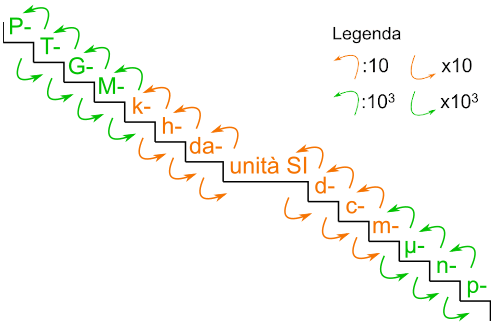
\includegraphics[width=.9\columnwidth]{img/multipli.png}
\end{figure}
\end{frame}

\section{Equivalenze}

\begin{frame}
\frametitle{Equivalenza tra udm (lunghezza e massa)}
Un'equivalenza esprime una stessa misura in due udm diverse (compatibili con la misura).{\pause} Ad esempio:

~

\begin{columns}
\begin{column}{0.4\textwidth}
\alert<3>{$ 1,75 \, m = 175 \, cm $

~

$ 3 \, mg = 30 \, cg $}
\end{column}
\begin{column}{0.4\textwidth}
\alert<4>{$ 428 \, mm = 42,8 \, cm $

~

$ 153 \, g = 1,53 \, hg $}
\end{column}
\end{columns}

~\pause

Quindi:
\begin{itemize}
  \item \alert<3>{se la seconda udm è 10, 100, \ldots volte più piccola della prima, si moltiplica la misura per 10, 100, \ldots};
  \item \alert<4>{se la seconda udm è 10, 100, \ldots volte più grande della prima, si divide la misura per 10, 100, \ldots}
\end{itemize}
\end{frame}




\begin{frame}
\frametitle{Esercizi (1)}
\begin{enumerate}
  \item Converti le seguenti lunghezze in metri:
  \begin{multicols}{2}
    \begin{itemize}
        \item $ 2,5 \, km = \ldots \, m $
        \item $ 800 \, mm = \ldots \, m $
        \item $ 7\,600\,000 \, nm = \ldots \, m $
        \item $ 3,4 \, cm = \ldots \, m $
    \end{itemize}
  \end{multicols}
  \item Converti le seguenti masse in chilogrammi:
  \begin{multicols}{2}
    \begin{itemize}
        \item $ 650 \, g = \ldots \, kg $
        \item $ 18,07 \, mg = \ldots \, kg $
        \item $ 45 \, g = \ldots \, kg $
        \item $ 9,23 \, hg = \ldots \, kg $
    \end{itemize}
  \end{multicols}
  \item Un lottatore di sumo ha una massa pari a $ 230,5 \, kg $. Il suo avversario ha una massa inferiore di $ 15\,200 \, g $.
  
  Qual è la massa dell'avversario?
\end{enumerate}
\end{frame}



\begin{frame}
\frametitle{Equivalenza tra udm (area)}
L'area si misura con una udm derivata, il \alert<1>{metro quadrato}:
\begin{center}
$ 1 \, m^2 = 1 \, m \cdot m $
\end{center}\pause
Notiamo che:
\begin{center}
$ 1 \, cm^2 = 1 \, cm \cdot cm = \dfrac{1}{10} \, m \cdot \dfrac{1}{10} \, m  = \dfrac{1}{10\,000} \, m^2$
\end{center}\pause
In pratica, \alert<3>{per le unità di area, si fanno sempre il ``doppio dei salti''} rispetto a quanti ne faremmo per le unità di lunghezza.
\begin{center}
$ 1 \, m^2 = 10\,000 \, cm^2 $
\end{center}
\end{frame}



\begin{frame}
\frametitle{Esercizi (2)}
\begin{enumerate}
  \item Converti le seguenti misure di area nella udm indicata:
  \begin{multicols}{2}
    \begin{itemize}
        \item $ 100 \, cm^2 = \ldots \, m^2 $
        \item $ 3,7 \, km^2 = \ldots \, mm^2 $
        \item $ 25 \, dm^2 = \ldots \, m^2 $
        \item $ 8,4 \, dm^2 = \ldots \, cm^2 $
    \end{itemize}
  \end{multicols}
  \item Il giardino della casa di Dario è rettangolare: è lungo $ 0,020 \, km $ e largo $ 1\,500 \, cm $.
  
  Quanto misura l'area del giardino in $ m^2 $?
\end{enumerate}
\end{frame}




\begin{frame}
\frametitle{Equivalenza tra udm (volume)}
Il volume si misura con una udm derivata, il \alert<1>{metro cubo}:
\begin{center}
$ 1 \, m^3 = 1 \, m \cdot m \cdot m $
\end{center}\pause
Valgono le stesse osservazioni fatte per le unità di area, ma qui \alert<2>{si fanno sempre il ``triplo dei salti''} rispetto a quanti ne faremmo per le unità di lunghezza.
\begin{center}
$ 1 \, m^3 = 1\,000\,000 \, cm^2 $
\end{center}\pause
Ricordiamo inoltre che \alert{$ 1 \, L = 1 \, dm^3 $} (un cubo di lato $ 10 \, cm $ contiene esattamente un litro di acqua).
\end{frame}


\begin{frame}
\frametitle{Esercizi (3)}
\begin{enumerate}
  \item Converti le seguenti misure di volume nella udm indicata:
  \begin{multicols}{2}
    \begin{itemize}
        \item $ 2 \, dm^3 = \ldots \, cm^3 $
        \item $ 415\,190 \, mm^3 = \ldots \, m^3 $
        \item $ 187 \, dL = \ldots \, dm^3 $
        \item $ 1\,868 \, L = \ldots \, m^3 $
    \end{itemize}
  \end{multicols}
  \item In laboratorio devi prelevare da un rubinetto $ 1,41 \, L $ di acqua. Hai a disposizione un cilindro da mezzo litro, un becher da $ 12 \, cL $ e un cucchiaio da $ 5 \, cL $.
  
  Quante volte utilizzi il cilindro, il becher e il cucchiaio per ottenere il volume desiderato?
\end{enumerate}
\end{frame}




\begin{frame}
\frametitle{Equivalenza tra udm (tempo)}
I sottomultipli del secondo funzionano come le altre udm.

~

I multipli del secondo invece sono i minuti, le ore, i giorni e gli anni.

~

\begin{columns}
\begin{column}{0.4\textwidth}
$ 1 \, min = 60 \, s $

~

$ 1 \, d = 24 \, h = 86\,400 \, s $
\end{column}
\begin{column}{0.4\textwidth}
$ 1 \, h = 60 \, min = 3\,600 \, s $

~

$ 1 \, y = 365 \, d = 31\,536\,000 \, s$
\end{column}
\end{columns}
\end{frame}



\begin{frame}
\frametitle{Esercizi (4)}
\begin{enumerate}
  \item Converti le seguenti misure di tempo nella udm indicata:
  \begin{multicols}{2}
    \begin{itemize}
        \item $ 12,5 \, h = \ldots \, s $
        \item $ 18 \, h \,\, 50 \, min = \ldots \, s $
    \end{itemize}
  \end{multicols}
  \item Il 12 Novembre Amelia afferma che mancano $ 17 \, 280 \, min $ al suo compleanno.
  
  In che giorno Amelia compie gli anni?
\end{enumerate}
\end{frame}


\section{Notazione}

\begin{frame}
\frametitle{Numeri scomodi}
Negli esercizi precedenti abbiamo incontrato numeri come:
\begin{center}
$ 3,7 \, km^2 = 3700000000000 \, mm^2 $

~
$ 415190 \, mm^3 = 0,000415190 \, m^3$
\end{center}\pause
Nelle scienze si utilizza una scrittura più agevole, che sfrutta le \alert<2->{potenze di 10}.

\begin{center}
\colorbox{blue!30}{$10^n = \underbrace{\hbox{$10 \times 10 \times \ldots \times 10$}}_{\hbox{$ n $ volte}}$}\pause~~~~~~~\colorbox{blue!30}{$10^0 = 1$}\pause~~~~~~~\colorbox{blue!30}{$10^{-n} = \dfrac{1}{10^n}$}
\end{center}
Occhio alle potenze negative: $ 10^{-3} = \dfrac{1}{10^3} = \dfrac{1}{1000} = $ un millesimo.
\end{frame}


\begin{frame}
\frametitle{Calcolo con le potenze di 10}
Valgono le solite proprietà delle potenze:
  \begin{center}
  \colorbox{blue!30}{$10^{a} \times 10^b = 10^{a\alert{+}b}$}~~~~~~~~\colorbox{blue!30}{$\dfrac{10^{a}}{10^b} = 10^{a\alert{-}b}$}~~~~~~~~\colorbox{blue!30}{$\left( 10^a \right)^b = 10^{a\alert{\cdot}b}$}
  \end{center}\pause
  Prova a calcolare:
  
  ~
  
  \begin{itemize}
    \item $ \dfrac{10^3 \times 10^{-7}}{10^{-2}} = \pause 10^{3+(-7) - (-2)} =\pause  10^{-2} $\pause
    
    ~
    
    \item $ \dfrac{\left( 10^{-1} \times 10^{9} \right)^2 \times 10^{-12}}{10^7 \times 10^{-1}} = $
  \end{itemize}
\end{frame}



\begin{frame}
\frametitle{Notazione scientifica}
Quando esprimiamo un numero in notazione scientifica (o esponenziale) utilizziamo:
\begin{itemize}
  \item un numero con \alert{una sola cifra intera} (lasciamo il resto nei decimali);\pause
  \item \alert{una potenza di 10}.
\end{itemize}\pause

~

Ad esempio:
\begin{itemize}
  \item $ 1,2305 \times 10^3 $ è in notazione scientifica;
  \item $ 12,305 \times 10^2 $ non lo è.
\end{itemize}
\end{frame}

\begin{frame}
\frametitle{Esercizi (5)}
\begin{center}
$ 1\alert{\overleftarrow{251}} ,4 = 1,2514 \times 10^{\alert{3}} $~~~~~~~$ 0,\alert{\overrightarrow{0007}}32 = 7,32 \times 10^{\alert{-4}} $
\end{center}
\begin{enumerate}
  \item Scrivi i seguenti numeri in notazione scientifica:
  \begin{multicols}{2}
    \begin{itemize}
        \item $ 12,5 $
        \item $ 0,005478 $
        \item $ 94723,56 $
        \item $ 0,55 $
    \end{itemize}
  \end{multicols}
  \item Scrivi i seguenti numeri in notazione scientifica:
  \begin{multicols}{2}
    \begin{itemize}
        \item $ 5675 \times 10^{-1} $
        \item $ 98 \times 10^{23} $
        \item $ 0,045 \times 10^2 $
        \item $ 0,45834 \times 10^{-4} $
    \end{itemize}
  \end{multicols}
\end{enumerate}
\end{frame}


\begin{frame}
\frametitle{Potenze di 10 e unità di misura}
La notazione scientifica è assai comoda nella conversione di una misura da una udm all'altra.\pause

~

Ad esempio, se $ 1 \, km = 1 \times 10^{3} \, m $, allora:
\begin{center}
$ 52,4 \, km = 52,4 \times 10^{3} \, m = 5,24 \times 10^{4} \, m $
\end{center}\pause

~

Inoltre, se $ 1 \, \mu m = 1 \times 10^{-6} \, m $, allora:
\begin{center}
$ 0,44 \, \mu m = 0,44 \times 10^{-6} \, m = 4,4 \times 10^{-7} \, m $
\end{center}
\end{frame}


\begin{frame}
\frametitle{Esercizi (6)}
\begin{enumerate}
  \item Converti le seguenti misure in metri utilizzando la notazione scientifica:
  \begin{multicols}{2}
    \begin{itemize}
        \item $ 8,1 \, km = \ldots \, m $
        \item $ 930 \, mm = \ldots \, m $
        \item $ 6\,700\,000 \, nm = \ldots \, m $
        \item $ 9,9 \, cm = \ldots \, m $
    \end{itemize}
  \end{multicols}
  \item Converti le seguenti masse in chilogrammi utilizzando la notazione scientifica:
  \begin{multicols}{2}
    \begin{itemize}
        \item $ 650 \, g = \ldots \, kg $
        \item $ 18,07 \, mg = \ldots \, kg $
        \item $ 4500 \, g = \ldots \, kg $
        \item $ 0,23 \, hg = \ldots \, kg $
    \end{itemize}
  \end{multicols}
\end{enumerate}
\end{frame}



\section{Proporzionalità}

\begin{frame}
\frametitle{Legami tra quantità}
Quando facciamo Fisica, cerchiamo di trovare e di esprimere (matematicamente) la \alert<1>{relazione che sussiste tra più quantità misurate}.\pause

~

Parliamo di:
\begin{itemize}
  \item \alert<2>{proporzionalità diretta} tra due quantità $ x $ e $ y $ quando, all'aumentare di $ x $, aumenta anche $ y $;\pause
  \item \alert<3>{proporzionalità inversa} tra $ x $ e $ y $ quando, all'aumentare di $ x $, diminuisce $ y $;
\end{itemize}
\end{frame}


\begin{frame}
\frametitle{Proporzionalità diretta (lineare)}
Immaginiamo dei quadrati con lati diversi e calcoliamo i loro perimetri:

~

\begin{columns}
\begin{column}{0.4\textwidth}
\centering
\begin{tabular}{c|c}
\textbf{lato} $ [m] $ & \textbf{perimetro} [m] \\\rule{0pt}{4ex}
$ 1 $ & $ 4 $ \\\rule{0pt}{3ex}
$ 2 $ & $ 8 $ \\\rule{0pt}{3ex}
$ 3 $ & $ 12 $ \\\rule{0pt}{3ex}
$ 4 $ & $ 16 $ \\\
\end{tabular}
~

$ p = 4\cdot l $
\end{column}
\begin{column}{0.4\textwidth}
\pause Notiamo che il \alert<2>{se il lato raddoppia, raddoppia anche il perimetro; se il lato triplica, triplica anche il perimetro}, ecc.\pause

~

Parliamo in questo caso di \alert<3>{proporzionalità diretta lineare}.
\end{column}
\end{columns}
\end{frame}

\begin{frame}
\frametitle{Formula e grafico della proporzionalità lineare}
\begin{block}{Proporzionalità diretta lineare}
Due variabili direttamente proporzionali $ x $ e $ y $ sono legate dalle relazioni:
\begin{center}
\colorbox{blue!30}{$ y = k \cdot x $}~~~~~~~~~\colorbox{blue!30}{$ \dfrac{y}{x} = k $}
\end{center}\pause
\end{block}

\begin{columns}
\begin{column}{0.4\textwidth}
\begin{figure}\centering
\begin{tikzpicture}[scale=0.3]
\draw [->] (-1,0) -- (7,0);
\draw [->] (0,-1) -- (0,7);
\node [below] at (7,0) {$ x $};
\node [below,blue] at (2,9) {$ k_{blu} $};
\node [below] at (3.6,8.8) {$ > $};
\node [below,red] at (5.6,9) {$ k_{rossa} $};
\node [left] at (0,7) {$ y $};
\draw [thick,red] (0,0) -- (7,3);
\draw [thick,blue] (0,0) -- (7,6);
\draw [red,fill=red] (2,6/7) circle [radius=.1];
\draw [red,fill=red] (4,12/7) circle [radius=.1];
\draw [red,fill=red] (6,18/7) circle [radius=.1];
\draw [blue,fill=blue] (2,12/7) circle [radius=.1];
\draw [blue,fill=blue] (4,24/7) circle [radius=.1];
\draw [blue,fill=blue] (6,36/7) circle [radius=.1];
\end{tikzpicture}
\end{figure}
\end{column}
\begin{column}{0.4\textwidth}
Il grafico è una \alert{retta passante per l'origine}, la cui pendenza dipende dal valore di $ k $ (costante di proporzionalità).
\end{column}
\end{columns}
\end{frame}




\begin{frame}
\frametitle{Proporzionalità inversa}
Immaginiamo dei rettangoli di area $ 12 \, m^2 $ e calcoliamo l'altezza in funzione della base:

~

\begin{columns}
\begin{column}{0.4\textwidth}
\centering
\begin{tabular}{c|c}
\textbf{b} $ [m] $ & \textbf{h} [m] \\\rule{0pt}{4ex}
$ 2 $ & $ 6 $ \\\rule{0pt}{3ex}
$ 3 $ & $ 4 $ \\\rule{0pt}{3ex}
$ 4 $ & $ 3 $ \\\rule{0pt}{3ex}
$ 6 $ & $ 2 $ \\\
\end{tabular}

~

$ b \cdot h = A $
\end{column}
\begin{column}{0.4\textwidth}
\pause Notiamo che il \alert<2>{il prodotto rimane costante, e se una aumenta l'altra diminuisce}.\pause

~

Parliamo in questo caso di \alert<3>{proporzionalità inversa}.
\end{column}
\end{columns}
\end{frame}




\begin{frame}
\frametitle{Formula e grafico della proporzionalità inversa}
\begin{block}{Proporzionalità inversa}
Due variabili inversamente proporzionali $ x $ e $ y $ sono legate dalle relazioni:
\begin{center}
\colorbox{blue!30}{$ x \cdot y = k $}~~~~~~~~~\colorbox{blue!30}{$ y = \dfrac{k}{x} $}
\end{center}\pause
\end{block}

\begin{columns}
\begin{column}{0.4\textwidth}
\begin{figure}\centering
\begin{tikzpicture}[scale=0.3]
\draw [->] (-1,0) -- (7,0);
\draw [->] (0,-1) -- (0,7);
\node [below] at (7,0) {$ x $};
\node [left] at (0,7) {$ y $};
\draw[smooth, orange, thick, domain=0.45:6.6, samples=50] plot 
({\x},{    3*(\x)^-1           });
\draw [orange,fill=orange] (3/4,4) circle [radius=.1];
\draw [orange,fill=orange] (.5,6) circle [radius=.1];
\draw [orange,fill=orange] (2,3/2) circle [radius=.1];
\draw [orange,fill=orange] (4,3/4) circle [radius=.1];
\draw [orange,fill=orange] (6,3/6) circle [radius=.1];
\end{tikzpicture}
\end{figure}
\end{column}
\begin{column}{0.4\textwidth}
Il grafico è un \alert{ramo di iperbole}.
\end{column}
\end{columns}
\end{frame}

\begin{frame}
\frametitle{Formula e grafico della proporzionalità quadratica}
\begin{block}{Proporzionalità diretta quadratica}
Due variabili $ x $ e $ y $ con proporzionalità quadratica sono legate dalla relazione:
\begin{center}
\colorbox{blue!30}{$ y = k \cdot x^2 $}
\end{center}\pause
\end{block}

\begin{columns}
\begin{column}{0.4\textwidth}
\begin{figure}\centering
\begin{tikzpicture}[scale=0.3]
\draw [->] (-1,0) -- (7,0);
\draw [->] (0,-1) -- (0,7);
\node [below] at (7,0) {$ x $};
\node [left] at (0,7) {$ y $};
\draw[smooth, green, thick, domain=0:6, samples=50] plot 
({\x},{    .25*(\x)^2           });
\draw [green,fill=green] (2,1) circle [radius=.1];
\draw [green,fill=green] (4,4) circle [radius=.1];
\draw [green,fill=green] (6,9) circle [radius=.1];
\end{tikzpicture}
\end{figure}
\end{column}
\begin{column}{0.4\textwidth}
Il grafico è un \alert{ramo di parabola}.
\end{column}
\end{columns}
\end{frame}



\begin{frame}
\frametitle{Cosa dice una formula}
Una formula afferma che \alert{tra certe quantità esiste una relazione} (ad esempio di proporzionalità diretta o inversa).\pause

~

Ad esempio, per un triangolo:
\begin{itemize}
  \item la formula: \begin{center}
  $ p = l_1 + l_2 + l_3 $
  \end{center}
  ci dice che il perimetro è la somma di tutti i lati;\pause
  \item la formula:\begin{center}
  $ A = \dfrac{1}{2} \cdot b \cdot h $
  \end{center} ci dice che l'area è direttamente proporzionale all'altezza (e alla base).
\end{itemize}
\end{frame}


\begin{frame}
\frametitle{Riconoscere una proporzionalità}
Dobbiamo individuare la \alert<1>{struttura della formula} e la posizione delle quantità tra le quali vogliamo leggere la proporzionalità.\pause
\begin{columns}
\begin{column}{0.4\textwidth}
\begin{center}
\textbf{Diretta}

\vspace{.3cm}

$ \textcolor{orange}{y} = k \textcolor{orange}{x} $~~~~~~~~~$ \dfrac{\textcolor{orange}{y}}{\textcolor{orange}{x}} = k $
\end{center}
\end{column}
\begin{column}{0.4\textwidth}
\begin{center}
\textbf{Inversa}

\vspace{.3cm}

$ \textcolor{purple}{x} \textcolor{purple}{y} = k $~~~~~~~~~$ \textcolor{purple}{y} = \dfrac{k}{\textcolor{purple}{x}} $
\end{center}
\end{column}
\end{columns}\pause

~

~

Ad esempio, in: ~~~~~~~~~~~~~~
$ \dfrac{\alert<3,6>{p}\alert<4-6>{V}}{\alert<5,7>{T}} = \alert<3-4,7>{k} $

\begin{itemize}
  \item $ p $ è \alert<3>{direttamente proporzionale} a $ k $;\pause
  \item $ V $ è \alert<4>{direttamente proporzionale} a $ k $;\pause
  \item $ V $ è \alert<5>{direttamente proporzionale} a $ T $;\pause
  \item $ p $ è \alert<6>{inversamente proporzionale} a $ V $\pause
  \item $ T $ è \alert<7>{inversamente proporzionale} a $ k $
\end{itemize}

\end{frame}




\begin{frame}
\frametitle{Esercizi (7)}
Completa inserendo ``direttamente/inversamente proporzionale'' nelle seguenti affermazioni.
\begin{enumerate}
  \item Nella formula:\begin{center}
  $ pV = nRT $
  \end{center}
  \begin{multicols}{2}
    \begin{itemize}
        \item $ p $ è \ldots \ldots \ldots a $ V $;
        \item $ p $ è \ldots \ldots \ldots a $ T $;
        \item $ T $ è \ldots \ldots \ldots a $ p $;
        \item $ T $ è \ldots \ldots \ldots a $ n $;
    \end{itemize}
  \end{multicols}
  \item Nella formula:\begin{center}
  $ F = k_0 \cdot \dfrac{q_1 q_2}{r^2} $
  \end{center}
  \begin{multicols}{2}
    \begin{itemize}
        \item $ F $ è \ldots \ldots \ldots a $ q_1 $;
        \item $ q_1 $ è \ldots \ldots \ldots a $ q_2 $;
        \item $ F $ è \ldots \ldots \ldots a $ r^2 $;
        \item $ q_2 $ è \ldots \ldots \ldots a $ r^2 $;
    \end{itemize}
  \end{multicols}
\end{enumerate}
\end{frame}


\section{Formule}



\begin{frame}
\frametitle{Le ``formule inverse''}
La relazione tra delle quantità può essere espressa in diversi modi, a seconda di ciò che siamo interessati a dire o a calcolare.\pause

~

Per un rettangolo, possiamo dire:
\begin{columns}
\begin{column}{0.45\textwidth}
\begin{center}
$ A = bh $
\end{center}
Ovvero, conoscendo base e altezza, possiamo calcolare l'area.\pause
\end{column}
\begin{column}{0.45\textwidth}
\begin{center}
$ h = \dfrac{A}{b} $
\end{center}
Ovvero, conoscendo area e base, possiamo calcolare l'altezza.\pause
\end{column}
\end{columns}

~

~

Non ha senso imparare una relazione e anche le sue ``inverse'': impariamo a \alert{manipolare le formule}!
\end{frame}


\begin{frame}
\frametitle{Premessa}
Con le formule di Fisica possiamo eseguire tutte le operazioni matematiche che conosciamo, come:
\begin{itemize}
  \item spostare un termine da una parte all'altra di una formula cambiandogli il segno;
  \begin{center}
  $ s = vt + s_0 ~~~~ \Longrightarrow ~~~~ s - s_0 = vt $
  \end{center}\pause
  \item moltiplicare e dividere entrambi i membri per una stessa quantità;
  \begin{center}
  $ K = \dfrac{1}{2}mv^2 ~~~~ \Longrightarrow ~~~~2K = mv^2 $
  \end{center}\pause
  \item estrarre la radice quadrata di entrambi i membri;
  \begin{center}
  $ K = \dfrac{1}{2}mv^2 ~~~~ \Longrightarrow ~~~~ v^2 = \dfrac{2K}{m} ~~~~ \Longrightarrow ~~~~ v = \sqrt{\dfrac{2K}{m}} $
  \end{center}
  \item ecc.
\end{itemize}
\end{frame}



\begin{frame}
\frametitle{1. Individuare la struttura}
Buona parte delle formule presentano (o vi possono essere ricondotte) la struttura:
\begin{center}
\Large \colorbox{blue!30}{$ \dfrac{A}{B} = \dfrac{C}{D}$}
\end{center}
\end{frame}

\begin{frame}
\frametitle{Esempio}
\begin{center}
\Large $ \dfrac{\textcolor{red}{A}}{\textcolor{blue}{B}} = \dfrac{\textcolor{orange}{C}}{\textcolor{teal}{D}}$
\end{center}

~

~

Riconosciamo la struttura in diverse formule:
\begin{columns}
\begin{column}{0.5\textwidth}
\begin{center}
$ d = \dfrac{m}{V} ~~~~ \Longrightarrow ~~~~ \dfrac{\textcolor{red}{d}}{\textcolor{blue}{1}} = \dfrac{\textcolor{orange}{m}}{\textcolor{teal}{V}} $
\end{center}\pause
\begin{center}
$ \omega = \dfrac{2 \pi}{T} ~~~~ \Longrightarrow ~~~~ \dfrac{\textcolor{red}{\omega}}{\textcolor{blue}{1}} = \dfrac{\textcolor{orange}{2\pi}}{\textcolor{teal}{T}} $
\end{center}\pause
\end{column}
\begin{column}{0.5\textwidth}
\begin{center}
$ F = ma ~~~~ \Longrightarrow ~~~~ \dfrac{\textcolor{red}{F}}{\textcolor{blue}{1}} = \dfrac{\textcolor{orange}{ma}}{\textcolor{teal}{1}} $
\end{center}\pause
\begin{center}
$ K = \dfrac{1}{2}mv^2 ~~~~ \Longrightarrow ~~~~ \dfrac{\textcolor{red}{K}}{\textcolor{blue}{1}} = \dfrac{\textcolor{orange}{mv^2}}{\textcolor{teal}{2}} $
\end{center}
\end{column}
\end{columns}
\end{frame}


\begin{frame}
\frametitle{2. Spostamenti ``a croce''}
Possiamo ora immaginare due binari, disposti a croce, lungo i quali possiamo liberamente spostare le quantità coinvolte:
\begin{figure}\centering
\begin{tikzpicture}[scale=0.3]
\node [below] at (0,0) {$ B $};
\node [above] at (0,0) {$ A $};
\node [below] at (5,0) {$ D $};
\node [above] at (5,0) {$ C $};
\draw [] (-.8,0) -- (.8,0);
\draw [] (4.2,0) -- (5.8,0);
\draw [] (2,.2) -- (3,.2);
\draw [] (2,-.2) -- (3,-.2);
\draw [<->,thick,red] (1,-1) -- (4,1);
\draw [<->,thick,blue] (1,1) -- (4,-1);
\end{tikzpicture}
\end{figure}\pause
In base a cosa vogliamo esprimere, possiamo modificare la struttura facendo ``scorrere'' le quantità lungo i binari, ad esempio:
  \begin{multicols}{2}
    \begin{itemize}
        \item $ A = \dfrac{B C}{D} $;\pause
        \item $ \dfrac{AD}{B} = C $;\pause
        \item $ \dfrac{AD}{C} = B $;\pause
        \item $ D = \dfrac{BC}{A} $;
    \end{itemize}
  \end{multicols}
\end{frame}

\begin{frame}
\frametitle{Esempio}
\begin{figure}\centering
\begin{tikzpicture}[scale=0.3]
\node [below] at (0,0) {$ B $};
\node [above] at (0,0) {$ A $};
\node [below] at (5,0) {$ D $};
\node [above] at (5,0) {$ C $};
\draw [] (-.8,0) -- (.8,0);
\draw [] (4.2,0) -- (5.8,0);
\draw [] (2,.2) -- (3,.2);
\draw [] (2,-.2) -- (3,-.2);
\draw [<->,thick,red] (1,-1) -- (4,1);
\draw [<->,thick,blue] (1,1) -- (4,-1);
\end{tikzpicture}
\end{figure}

Proviamo a modificare la formula:
\begin{center}
\alert{$ \dfrac{pV}{T} = k $}
\end{center}\pause
\begin{itemize}
  \item scambiando $ T $ e $ k $ otteniamo:\pause
  \begin{center}
  \alert<3>{$ T = \dfrac{pV}{k} $}
  \end{center}\pause
  \item spostando $ V $ e $ T $ otteniamo: \pause\begin{center}
  \alert<5>{$ p = \dfrac{kT}{V} $}
  \end{center}
\end{itemize}
\end{frame}


\begin{frame}
\frametitle{Esercizi (8)}
\begin{enumerate}
  \item Modifica $ F = G \dfrac{m_1 m_2}{r^2} $ in modo da esprimere:
  \begin{multicols}{2}
    \begin{itemize}
        \item $ G $;
        \item $ m_1 $;
        \item $ r^2 $;
        \item $ r $;
    \end{itemize}
  \end{multicols}
  \item Modifica $ v = \dfrac{mg}{6\pi \eta r} $ in modo da esprimere:
  \begin{multicols}{2}
    \begin{itemize}
        \item $ m $;
        \item $ g $;
        \item $ r $;
        \item $ 6 $;
    \end{itemize}
  \end{multicols}
\end{enumerate}
\end{frame}


\begin{frame}
\frametitle{Formule e linguaggio naturale}
Spesso \alert<1>{la relazione tra due quantità è espressa a parole}, senza utilizzare una formula.\pause

~

Per poter utilizzare gli strumenti che stiamo studiando, è necessario \alert<2>{esprimerla in linguaggio matematico}.\pause

~

\begin{itemize}
  \item ``Il \textcolor{red}{volume della scatola rossa} ($ v_r $) è il \textcolor{orange}{doppio} del \textcolor{blue}{volume della scatola blu} ($ v_b $)''
  \begin{center}
  $ \textcolor{red}{v_r} = \textcolor{orange}{2} \textcolor{blue}{v_b} $
  \end{center}\pause
  \item ``La massa \textcolor{red}{$ M $} si separa in due masse \textcolor{orange}{$ m_1 $} e \textcolor{blue}{$ m_2 $}''
    \begin{center}
  $ \textcolor{red}{M} = \textcolor{orange}{m_1} + \textcolor{blue}{m_2} $
  \end{center}
\end{itemize}
\end{frame}

\begin{frame}
\frametitle{Esercizi (9)}
\begin{enumerate}
  \item Esprimi le seguenti frasi in linguaggio matematico:
  
  ~

    \begin{itemize}
        \item ``alla carica $ Q_1 $ viene affiancata la carica $ Q_2 $, ottenendo la carica totale'';
        
        ~

        \item ``la massa della seconda scatola è il triplo della massa della prima scatola''.
        
        ~
        
        \item ``una macchina termica guadagna una quantità di energia $ L $; perde poi una quantità di energia $ Q $, rimanendo con $ 314 \, J $ di energia'';
        
        ~
        
        \item ``la pressione $ p $ e il volume $ V $ di un gas perfetto sono inversamente proporzionali''.
    \end{itemize}
\end{enumerate}
\end{frame}



\begin{frame}
\frametitle{Lavorare algebricamente}
Svolgere un esercizio di Fisica non richiede soltanto di ``applicare una formula'': dovremo a volte \alert<1>{ottenere la formula} che ci serve.\pause

~

È spesso necessario \alert<2>{collegare tra loro due o più formule} e modificare poi ciò che si ottiene utilizzando il \alert<2>{calcolo letterale}.\pause

~

Ad esempio, se sappiamo che:
\begin{center}
  $ F = ma $ ~~~~~ e ~~~~~ $ F = -kx $
\end{center}
e vogliamo trovare $a$,{\pause} possiamo ottenere:
\begin{center}
  $ ma = -kx $\pause

  ~

  $ a = -\dfrac{kx}{m} $
\end{center}
\end{frame}



\begin{frame}
\frametitle{Esercizi (10)}
\begin{enumerate}
  \item Sapendo che:
  \begin{center}
    $ U = mgh $, ~~~~~ $ U = \dfrac{1}{2}mv^2 $
  \end{center}
  trova una formula per esprimere $ h $ in funzione di $ g $ e di $ v $.

  ~

  \item Sapendo che:
  \begin{center}
    $ pV = nRT $, ~~~~~$ V = l^3 $,~~~~~ $ p = \dfrac{F}{S} $, ~~~~~$ S = l^2 $,~~~~~ $ F = ma $
  \end{center}
  trova una formula per esprimere $ m $ in funzione di $ n $, $ R $, $T$, $ a $ e $ l $.
\end{enumerate}
\end{frame}



\section{Percentuali}

\begin{frame}
\frametitle{Cosa sono le percentuali}
Troveremo spesso espressioni come:
\begin{center}
``La velocità dell'automobile aumenta del $ 17\% $.''

``Il $ 75\% $ dell'energia viene dissipata.''

``Il $ 53\% $ del cubo di legno è immerso in acqua.''\pause
\end{center}

~

\alert{Una percentuale è una frazione con denominatore $ 100 $.}
\begin{center}
$ 3\% = \dfrac{3}{100} = 0,03 $~~~~~~~$ 54\% = \dfrac{54}{100} = 0,54 $~~~~~~~$ 122\% = \dfrac{122}{100} = 1,22 $
\end{center}
\end{frame}

\begin{frame}
\frametitle{Esprimere informazioni con le percentuali}
\begin{center}
``La \textcolor{orange}{velocità finale} è il \textcolor{cyan}{$ 76\% $} di quella \textcolor{magenta}{iniziale}.''

$ \Downarrow  $

$ \textcolor{orange}{v_f} = \textcolor{cyan}{\dfrac{76}{100}}\textcolor{magenta}{v_i} $~~~~~~~$ \textcolor{orange}{v_f} = \textcolor{cyan}{0,76} \textcolor{magenta}{v_i} $
\end{center}\pause

~

~

\begin{center}
``La pressione \textcolor{orange}{aumenta} del $ \textcolor{cyan}{36\%} $.''

$ \Downarrow  $

$ p_f = p_i \textcolor{orange}{+} \textcolor{cyan}{0,36}p_i = (1+0,36)p_i  $\pause

~

$ p_f = 1,36p_i $
\end{center}

\end{frame}


\begin{frame}
\frametitle{Esercizi (11)}
\begin{enumerate}
  \item Esprimi le seguenti informazioni in linguaggio matematico, usando le percentuali:
        
  ~
        
    \begin{itemize}
        \item ``il volume finale è il 75\% del volume iniziale'';

        ~
        
        \item ``l'altezza del rettangolo è il $ 91\% $ della base''; 
        
        ~
      
        \item ``l'energia aumenta del 33\%''.
        
        ~
        
        \item ``la pressione diminuisce del $ 13\% $''.
    \end{itemize}
\end{enumerate}
\end{frame}


\begin{frame}
\frametitle{Calcolo di una percentuale}
Per calcolare una percentuale possiamo anche impostare la classica \alert{proporzione}.\pause

~

\begin{center}
``il $ 15\% $ di $ 76 \, kg $''

~

~

$\dfrac{x}{76 \, kg} = \dfrac{15}{100}  $\pause

~

~

$ x = \dfrac{15}{100}\cdot 76 \, kg= 0,15\cdot 76 \, kg = 11,4 \, kg $
\end{center}
\end{frame}


\begin{frame}
\frametitle{Esercizi (12)}
\begin{enumerate}
  \item Calcola le seguenti percentuali:
  
  ~
        
    \begin{itemize}
        \item il $ 78\% $ di $ 3546 \, J $ di energia;

        ~

        \item l'$ 1\% $ di $ 97 \, m^3 $;
        
        ~
        
        \item il $ 25\% $ di $ 80 \, s $;
        
        ~
        
        \item il $ 150\% $ di $ 50 \, kg $;
        
        ~
        
        \item il $ 23\% $ del $ 57\% $ di $ 236 \, m^2 $.
    \end{itemize}
\end{enumerate}
\end{frame}

\section{Calcoli}

\begin{frame}
\frametitle{Somme e sottrazioni}
Somme e sottrazioni possono essere eseguite:
\begin{itemize}
  \item solo tra quantità espresse con \alert<1-2>{la stessa udm};\pause
  \item solo tra quantità espresse con \alert<2>{la stessa potenza di 10}.
\end{itemize}\pause

~

Esempio:
\begin{center}
$ (3,45 \times 10^3 \,  \alert<3>{kg}) + (50,1 \times 10^2 \,  \alert<3>{kg}) = $\pause

\vspace{.3cm}

$ (3,45 \times \alert<4>{10^3} \, kg) + (5,01 \times \alert<4>{10^3} \, kg) =  $\pause

\vspace{.3cm}

$ \alert<5>{8,46 \times 10^3 \, kg} $
\end{center}
\end{frame}


\begin{frame}
\frametitle{Esercizi (13)}
\begin{enumerate}
  \item Esegui i seguenti calcoli:
  \begin{multicols}{2}
    \begin{itemize}
        \item $ 22,3 \times 10^{1} + 22 $;
        
        ~

        \item $ 22,3 \times 10^{1} + 22 \times 10^{2} $;
        \item $ 5,345 \times 10^{3} - 990 \times 10^{-1} $;
        
        ~

        \item $ 1 \times 10^{2} - 1 \times 10^{1} $;
    \end{itemize}
  \end{multicols}
\end{enumerate}
\end{frame}


\begin{frame}
\frametitle{Moltiplicazioni e divisioni}
Moltiplicazioni e divisioni possono essere eseguite:
\begin{itemize}
  \item tra quantità con \alert<1-2>{udm qualsiasi};\pause
  \item tra quantità con \alert<2>{potenze di 10 qualsiasi}.\pause
\end{itemize}

~

Il modo migliore è \alert{lavorare separatamente} su:
\begin{columns}
\begin{column}{0.4\textwidth}
\begin{enumerate}
  \item \textcolor{orange}{parte numerica};
  \item \textcolor{cyan}{potenza di 10};
  \item \textcolor{magenta}{udm}.
\end{enumerate}
\end{column}
\begin{column}{0.4\textwidth}
$ \textcolor{orange}{3,04} \times \textcolor{cyan}{10^2} \, \textcolor{magenta}{kg} $
\end{column}
\end{columns}

\end{frame}

\begin{frame}
\frametitle{Esempio}
Sapendo che:
\begin{multicols}{2}
  \begin{itemize}
      \item $ m = 3,22 \times 10^2 \, kg $;
      \item $ g = 9,81 \, \frac{N}{kg} $;
  \end{itemize}
\end{multicols}
calcoliamo \alert{$ P = mg $}.\pause
\begin{center}
$ P = (\textcolor{orange}{3,22} \times \textcolor{cyan}{10^2} \, \textcolor{magenta}{\cancel{kg}}) \cdot \left(\textcolor{orange}{9,81} \, \textcolor{magenta}{\dfrac{N}{\cancel{kg}}}\right) =\pause \textcolor{orange}{31,6} \times \textcolor{cyan}{10^2} \, \textcolor{magenta}{N} =\pause \textcolor{orange}{3,16} \times \textcolor{cyan}{10^3} \, \textcolor{magenta}{N}  $
\end{center}

\end{frame}


\begin{frame}
\frametitle{Esempio}
Sapendo che: 
\begin{multicols}{2}
  \begin{itemize}
    \item $ k = 9 \times 10^9 \, \frac{Nm^2}{C^2} $;
    
    ~

    \item $ q_1 = q_2 = 2 \times 10^{-6} \, C $;
    \item $ r = 1,2 \times 10^{-1} \, m $;
    
    ~
  \end{itemize}
\end{multicols}
calcoliamo \alert{$ F = k \dfrac{q_1 q_2}{r^2} $}.\pause
\begin{center}
$ F = \left(\textcolor{orange}{9} \times \textcolor{cyan}{10^9} \, \textcolor{magenta}{\dfrac{Nm^2}{C^2}}\right) \dfrac{(\textcolor{orange}{2} \times \textcolor{cyan}{10^{-6}} \, \textcolor{magenta}{C})(\textcolor{orange}{2} \times \textcolor{cyan}{10^{-6}} \, \textcolor{magenta}{C})}{(\textcolor{orange}{1,2} \times \textcolor{cyan}{10^{-1}} \, \textcolor{magenta}{m})^2} = $\pause

~

~

$ = \left(\textcolor{orange}{9} \times \textcolor{cyan}{10^9} \, \textcolor{magenta}{\dfrac{N\cancel{m^2}}{\cancel{C^2}}}\right) \dfrac{(\textcolor{orange}{4} \times \textcolor{cyan}{10^{-12}} \, \textcolor{magenta}{\cancel{C^2}})}{(\textcolor{orange}{1,44} \times \textcolor{cyan}{10^{-2}} \, \textcolor{magenta}{\cancel{m^2}})} = \pause\left(\textcolor{orange}{\dfrac{9 \cdot 4}{1,44}} \times \textcolor{cyan}{10^{9-12+2}} \, \textcolor{magenta}{N}\right) = $\pause

~

~

$ = \textcolor{orange}{25} \times \textcolor{cyan}{10^{-1}} \, \textcolor{magenta}{N} = \pause\textcolor{orange}{2,5} \, \textcolor{magenta}{N} $
\end{center}
\end{frame}


\begin{frame}
\frametitle{Esercizi (14)}
\begin{enumerate}
  \item Sapendo che \textcolor{blue}{$ m = 2,8 \times 10^2 \, kg $} e che \textcolor{purple}{$ a = 8,1 \times 10^{-1} \, \frac{N}{kg} $}, calcola $ F = \textcolor{blue}{m}\textcolor{purple}{a} $.
  
  ~

  \item Sapendo che $ m = 2,8 \times 10^2 \, kg $ e che $ v = 1,2 \times 10^1 \, \frac{m}{s} $, calcola $ K = \frac{1}{2} mv^2 $ (ricorda che $ \frac{kg \cdot m^2}{s^2} = J $).
  
  ~

  \item Usa la formula $ K = \dfrac{1}{2}mv^2 $ per calcolare:
    \begin{itemize}
        \item il valore di $ K $ quando $ m= 5,4 \, kg $ e $ v = 3 \, \frac{m}{s} $;
        \item il valore di $ m $ quando $ K = 400 \, J $ e $ v = 2,2 \, \frac{m}{s} $;
        \item il valore di $ v $ quando $ K = 3,8 \times 10^3 \, J $ e $ m = 9,2 \, kg $.
    \end{itemize}
\end{enumerate}
\end{frame}





\section{Precisione}

\begin{frame}
\frametitle{Misure ed errori}
Sappiamo che la Fisica si occupa di \alert<1>{quantità misurabili}.\pause

~

Ogni misura effettuata può essere più o meno precisa:

~

\begin{center}
``Il Monte Everest è alto \alert{$ 8848 \, m $}.''

~

~

``Il Monte Everest è alto \alert{$ 8848,43 \, m $}.''
\end{center}
\end{frame}


\begin{frame}
\frametitle{Cifre significative}
Scrivendo una misura utilizziamo un certo numero di \alert<1>{cifre significative}, che indicano con quanta precisione è stata effettuata la misura.\\~\pause
\begin{itemize}
  \item $ 1,2 $ ha due cifre significative;\pause
  \item $ 304 $ ha tre cifre significative;\pause
  \item $ 2,00 \times 10^{6} $ ha tre cifre significative.
\end{itemize}
\pause

~

\alert<5>{Tutte le cifre che usiamo per scrivere un numero sono significative, tranne gli zeri iniziali.}

~

\begin{itemize}
  \item $ 0,0377 $ ha tre cifre significative.
\end{itemize}
\end{frame}



\begin{frame}
\frametitle{Regole per le CS}
\begin{itemize}
  \item \textbf{Prodotti di numeri esatti per misure:} il risultato ha tante CS quante ne ha la misura di partenza;
\begin{center}
    $ 4 \cdot 3,67 \, m = 14,7 \, m $
  \end{center}~\pause
  \item \textbf{Somme e sottrazioni tra misure:} nel risultato sono significative tutte le cifre ottenute sommando o sottraendo cifre significative;
  \begin{center}
  $ 7,5 \, m + 1,23 \, m = 8,7 \, m $
  \end{center}~\pause
  \item \textbf{Prodotti e quozienti tra misure:} nel risultato si hanno tante CS quante se ne hanno nella misura che possiede meno CS.
  \begin{center}
  $ 4,5 \, kg \cdot 9,81 \, \dfrac{N}{kg} = 44 \, N $
  \end{center}
\end{itemize}
\end{frame}


\begin{frame}
\frametitle{Esercizi (15)}
\alert{Attenzione:} se la cifra successiva all'ultima CS da scrivere è 0, 1, 2, 3 o 4 si arrotonda per difetto, altrimenti per eccesso.

~

\begin{enumerate}
  \item Esegui i seguenti calcoli, esprimendo i risultati con il numero corretto di cifre significative.
  \begin{multicols}{2}
    \begin{itemize}
        \item $ 4 \cdot 3,04 \, kg $
        \item $ \pi \cdot 2,8 \, m $
        \item $ 7,52 \, s + 8,13 \, s $
        \item $ 7,52 \, s + 8,1 \, s $
        \item $ 7,52 \, s + 8 \, s $
        \item $ 8,0002 \, mg + 1,70 \, mg $
        \item $ 7,1 \, m^2 \cdot 9,15 \, m $
        \item $ 1,2 \, m \cdot 4,92 \, m $\\~
        \item $ \dfrac{15,02 \, m}{7,05 \, s} $\\~
        \item $ \dfrac{2,2 \times 10^2 \, m}{1,15 \times 10^1 s \cdot 3,33 \, s} $
    \end{itemize}
  \end{multicols}
\end{enumerate}
\end{frame}



\begin{frame}
\frametitle{Esercizi (16)}
\begin{enumerate}
  \item Avendo a disposizione le formule:
  
  ~

  \begin{center}
    $ F = ma $, ~~~~~$ F = k_0 \dfrac{q_1 q_2}{r^2} $,~~~~~ $ d = \dfrac{m}{V} $
  \end{center}

  ~

  e conoscendo i seguenti dati numerici:
  \begin{multicols}{2}
    $ d = 3,12 \times 10^{3} \, \dfrac{kg}{m^3}  $

    ~

    $ k_0 = 8,99 \times 10^{9} \, \dfrac{Nm^2}{C^2} $

    ~

    $ r = 2,00 \times 10^{-2} \, m $

    $ V = 5,20 \times 10^{-1} \, m^3 $

    ~

    $ a = 4,12 \, \dfrac{N}{kg} $

    ~

    $ q_1 = 3,00 \times 10^{-6} \, C $
  \end{multicols}
  calcola il valore di $ q_2 $ con il corretto numero di cifre significative.\hspace{\fill}[$ 9,91 \times 10^{-5} \, C $]
\end{enumerate}
\end{frame}





\end{document}
